% Created by tikzDevice version 0.12.3.1 on 2022-05-01 19:45:07
% !TEX encoding = UTF-8 Unicode
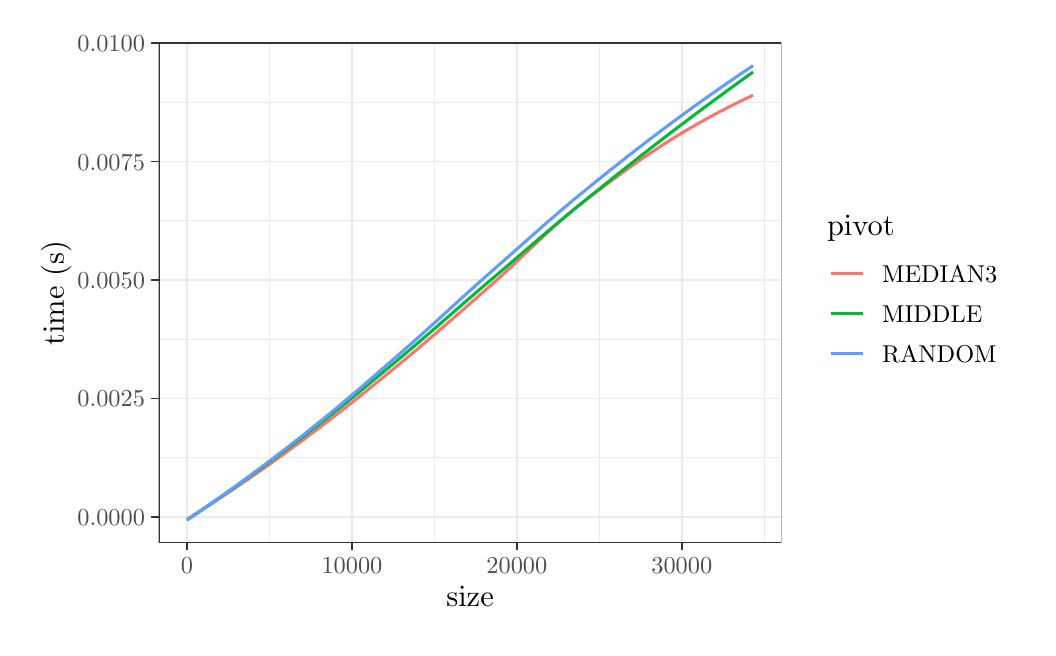
\begin{tikzpicture}[x=1pt,y=1pt]
\definecolor{fillColor}{RGB}{255,255,255}
\path[use as bounding box,fill=fillColor,fill opacity=0.00] (0,0) rectangle (361.35,216.81);
\begin{scope}
\path[clip] (  0.00,  0.00) rectangle (361.35,216.81);
\definecolor{drawColor}{RGB}{255,255,255}
\definecolor{fillColor}{RGB}{255,255,255}

\path[draw=drawColor,line width= 0.6pt,line join=round,line cap=round,fill=fillColor] (  0.00,  0.00) rectangle (361.35,216.81);
\end{scope}
\begin{scope}
\path[clip] ( 47.35, 30.69) rectangle (272.35,211.31);
\definecolor{fillColor}{RGB}{255,255,255}

\path[fill=fillColor] ( 47.35, 30.69) rectangle (272.35,211.31);
\definecolor{drawColor}{gray}{0.92}

\path[draw=drawColor,line width= 0.3pt,line join=round] ( 47.35, 61.39) --
	(272.35, 61.39);

\path[draw=drawColor,line width= 0.3pt,line join=round] ( 47.35,104.20) --
	(272.35,104.20);

\path[draw=drawColor,line width= 0.3pt,line join=round] ( 47.35,147.01) --
	(272.35,147.01);

\path[draw=drawColor,line width= 0.3pt,line join=round] ( 47.35,189.82) --
	(272.35,189.82);

\path[draw=drawColor,line width= 0.3pt,line join=round] ( 87.38, 30.69) --
	( 87.38,211.31);

\path[draw=drawColor,line width= 0.3pt,line join=round] (146.97, 30.69) --
	(146.97,211.31);

\path[draw=drawColor,line width= 0.3pt,line join=round] (206.57, 30.69) --
	(206.57,211.31);

\path[draw=drawColor,line width= 0.3pt,line join=round] (266.16, 30.69) --
	(266.16,211.31);

\path[draw=drawColor,line width= 0.6pt,line join=round] ( 47.35, 39.98) --
	(272.35, 39.98);

\path[draw=drawColor,line width= 0.6pt,line join=round] ( 47.35, 82.79) --
	(272.35, 82.79);

\path[draw=drawColor,line width= 0.6pt,line join=round] ( 47.35,125.60) --
	(272.35,125.60);

\path[draw=drawColor,line width= 0.6pt,line join=round] ( 47.35,168.41) --
	(272.35,168.41);

\path[draw=drawColor,line width= 0.6pt,line join=round] ( 47.35,211.22) --
	(272.35,211.22);

\path[draw=drawColor,line width= 0.6pt,line join=round] ( 57.58, 30.69) --
	( 57.58,211.31);

\path[draw=drawColor,line width= 0.6pt,line join=round] (117.18, 30.69) --
	(117.18,211.31);

\path[draw=drawColor,line width= 0.6pt,line join=round] (176.77, 30.69) --
	(176.77,211.31);

\path[draw=drawColor,line width= 0.6pt,line join=round] (236.37, 30.69) --
	(236.37,211.31);
\definecolor{drawColor}{RGB}{248,118,109}

\path[draw=drawColor,line width= 1.1pt,line join=round] ( 57.58, 39.18) --
	( 60.17, 40.80) --
	( 62.76, 42.45) --
	( 65.35, 44.11) --
	( 67.94, 45.79) --
	( 70.53, 47.49) --
	( 73.12, 49.22) --
	( 75.70, 50.96) --
	( 78.29, 52.72) --
	( 80.88, 54.49) --
	( 83.47, 56.29) --
	( 86.06, 58.10) --
	( 88.65, 59.94) --
	( 91.24, 61.79) --
	( 93.83, 63.67) --
	( 96.42, 65.56) --
	( 99.01, 67.46) --
	(101.60, 69.39) --
	(104.18, 71.32) --
	(106.77, 73.28) --
	(109.36, 75.26) --
	(111.95, 77.26) --
	(114.54, 79.28) --
	(117.13, 81.33) --
	(119.72, 83.39) --
	(122.31, 85.47) --
	(124.90, 87.56) --
	(127.49, 89.67) --
	(130.08, 91.78) --
	(132.67, 93.91) --
	(135.25, 96.04) --
	(137.84, 98.18) --
	(140.43,100.34) --
	(143.02,102.53) --
	(145.61,104.73) --
	(148.20,106.95) --
	(150.79,109.19) --
	(153.38,111.44) --
	(155.97,113.70) --
	(158.56,115.97) --
	(161.15,118.24) --
	(163.74,120.52) --
	(166.32,122.79) --
	(168.91,125.07) --
	(171.50,127.40) --
	(174.09,129.80) --
	(176.68,132.23) --
	(179.27,134.68) --
	(181.86,137.15) --
	(184.45,139.60) --
	(187.04,142.03) --
	(189.63,144.41) --
	(192.22,146.73) --
	(194.81,148.98) --
	(197.39,151.13) --
	(199.98,153.18) --
	(202.57,155.18) --
	(205.16,157.16) --
	(207.75,159.12) --
	(210.34,161.06) --
	(212.93,162.97) --
	(215.52,164.86) --
	(218.11,166.71) --
	(220.70,168.54) --
	(223.29,170.32) --
	(225.88,172.07) --
	(228.46,173.78) --
	(231.05,175.44) --
	(233.64,177.06) --
	(236.23,178.63) --
	(238.82,180.17) --
	(241.41,181.67) --
	(244.00,183.14) --
	(246.59,184.56) --
	(249.18,185.95) --
	(251.77,187.30) --
	(254.36,188.62) --
	(256.94,189.91) --
	(259.53,191.17) --
	(262.12,192.39);
\definecolor{drawColor}{RGB}{0,186,56}

\path[draw=drawColor,line width= 1.1pt,line join=round] ( 57.58, 38.90) --
	( 60.17, 40.63) --
	( 62.76, 42.38) --
	( 65.35, 44.15) --
	( 67.94, 45.93) --
	( 70.53, 47.74) --
	( 73.12, 49.56) --
	( 75.70, 51.39) --
	( 78.29, 53.25) --
	( 80.88, 55.11) --
	( 83.47, 57.00) --
	( 86.06, 58.90) --
	( 88.65, 60.82) --
	( 91.24, 62.75) --
	( 93.83, 64.71) --
	( 96.42, 66.67) --
	( 99.01, 68.65) --
	(101.60, 70.65) --
	(104.18, 72.65) --
	(106.77, 74.67) --
	(109.36, 76.72) --
	(111.95, 78.78) --
	(114.54, 80.87) --
	(117.13, 82.97) --
	(119.72, 85.09) --
	(122.31, 87.22) --
	(124.90, 89.37) --
	(127.49, 91.52) --
	(130.08, 93.68) --
	(132.67, 95.84) --
	(135.25, 98.01) --
	(137.84,100.18) --
	(140.43,102.38) --
	(143.02,104.60) --
	(145.61,106.83) --
	(148.20,109.07) --
	(150.79,111.33) --
	(153.38,113.59) --
	(155.97,115.84) --
	(158.56,118.10) --
	(161.15,120.34) --
	(163.74,122.57) --
	(166.32,124.78) --
	(168.91,126.97) --
	(171.50,129.17) --
	(174.09,131.38) --
	(176.68,133.60) --
	(179.27,135.82) --
	(181.86,138.04) --
	(184.45,140.25) --
	(187.04,142.46) --
	(189.63,144.66) --
	(192.22,146.84) --
	(194.81,149.00) --
	(197.39,151.13) --
	(199.98,153.24) --
	(202.57,155.34) --
	(205.16,157.43) --
	(207.75,159.51) --
	(210.34,161.59) --
	(212.93,163.65) --
	(215.52,165.71) --
	(218.11,167.76) --
	(220.70,169.80) --
	(223.29,171.82) --
	(225.88,173.83) --
	(228.46,175.84) --
	(231.05,177.82) --
	(233.64,179.80) --
	(236.23,181.76) --
	(238.82,183.71) --
	(241.41,185.65) --
	(244.00,187.58) --
	(246.59,189.50) --
	(249.18,191.40) --
	(251.77,193.30) --
	(254.36,195.19) --
	(256.94,197.06) --
	(259.53,198.93) --
	(262.12,200.78);
\definecolor{drawColor}{RGB}{97,156,255}

\path[draw=drawColor,line width= 1.1pt,line join=round] ( 57.58, 38.96) --
	( 60.17, 40.70) --
	( 62.76, 42.46) --
	( 65.35, 44.24) --
	( 67.94, 46.04) --
	( 70.53, 47.86) --
	( 73.12, 49.70) --
	( 75.70, 51.57) --
	( 78.29, 53.45) --
	( 80.88, 55.35) --
	( 83.47, 57.26) --
	( 86.06, 59.20) --
	( 88.65, 61.16) --
	( 91.24, 63.14) --
	( 93.83, 65.14) --
	( 96.42, 67.16) --
	( 99.01, 69.19) --
	(101.60, 71.24) --
	(104.18, 73.31) --
	(106.77, 75.39) --
	(109.36, 77.51) --
	(111.95, 79.65) --
	(114.54, 81.82) --
	(117.13, 84.00) --
	(119.72, 86.21) --
	(122.31, 88.44) --
	(124.90, 90.68) --
	(127.49, 92.92) --
	(130.08, 95.18) --
	(132.67, 97.43) --
	(135.25, 99.69) --
	(137.84,101.95) --
	(140.43,104.24) --
	(143.02,106.56) --
	(145.61,108.89) --
	(148.20,111.24) --
	(150.79,113.59) --
	(153.38,115.95) --
	(155.97,118.31) --
	(158.56,120.66) --
	(161.15,122.99) --
	(163.74,125.31) --
	(166.32,127.60) --
	(168.91,129.86) --
	(171.50,132.14) --
	(174.09,134.42) --
	(176.68,136.71) --
	(179.27,139.01) --
	(181.86,141.30) --
	(184.45,143.59) --
	(187.04,145.86) --
	(189.63,148.11) --
	(192.22,150.34) --
	(194.81,152.54) --
	(197.39,154.70) --
	(199.98,156.83) --
	(202.57,158.93) --
	(205.16,161.03) --
	(207.75,163.11) --
	(210.34,165.18) --
	(212.93,167.24) --
	(215.52,169.28) --
	(218.11,171.31) --
	(220.70,173.32) --
	(223.29,175.32) --
	(225.88,177.29) --
	(228.46,179.25) --
	(231.05,181.19) --
	(233.64,183.11) --
	(236.23,185.01) --
	(238.82,186.89) --
	(241.41,188.76) --
	(244.00,190.61) --
	(246.59,192.44) --
	(249.18,194.26) --
	(251.77,196.06) --
	(254.36,197.84) --
	(256.94,199.61) --
	(259.53,201.36) --
	(262.12,203.10);
\definecolor{drawColor}{gray}{0.20}

\path[draw=drawColor,line width= 0.6pt,line join=round,line cap=round] ( 47.35, 30.69) rectangle (272.35,211.31);
\end{scope}
\begin{scope}
\path[clip] (  0.00,  0.00) rectangle (361.35,216.81);
\definecolor{drawColor}{gray}{0.30}

\node[text=drawColor,anchor=base east,inner sep=0pt, outer sep=0pt, scale=  0.88] at ( 42.40, 36.95) {0.0000};

\node[text=drawColor,anchor=base east,inner sep=0pt, outer sep=0pt, scale=  0.88] at ( 42.40, 79.76) {0.0025};

\node[text=drawColor,anchor=base east,inner sep=0pt, outer sep=0pt, scale=  0.88] at ( 42.40,122.57) {0.0050};

\node[text=drawColor,anchor=base east,inner sep=0pt, outer sep=0pt, scale=  0.88] at ( 42.40,165.38) {0.0075};

\node[text=drawColor,anchor=base east,inner sep=0pt, outer sep=0pt, scale=  0.88] at ( 42.40,208.19) {0.0100};
\end{scope}
\begin{scope}
\path[clip] (  0.00,  0.00) rectangle (361.35,216.81);
\definecolor{drawColor}{gray}{0.20}

\path[draw=drawColor,line width= 0.6pt,line join=round] ( 44.60, 39.98) --
	( 47.35, 39.98);

\path[draw=drawColor,line width= 0.6pt,line join=round] ( 44.60, 82.79) --
	( 47.35, 82.79);

\path[draw=drawColor,line width= 0.6pt,line join=round] ( 44.60,125.60) --
	( 47.35,125.60);

\path[draw=drawColor,line width= 0.6pt,line join=round] ( 44.60,168.41) --
	( 47.35,168.41);

\path[draw=drawColor,line width= 0.6pt,line join=round] ( 44.60,211.22) --
	( 47.35,211.22);
\end{scope}
\begin{scope}
\path[clip] (  0.00,  0.00) rectangle (361.35,216.81);
\definecolor{drawColor}{gray}{0.20}

\path[draw=drawColor,line width= 0.6pt,line join=round] ( 57.58, 27.94) --
	( 57.58, 30.69);

\path[draw=drawColor,line width= 0.6pt,line join=round] (117.18, 27.94) --
	(117.18, 30.69);

\path[draw=drawColor,line width= 0.6pt,line join=round] (176.77, 27.94) --
	(176.77, 30.69);

\path[draw=drawColor,line width= 0.6pt,line join=round] (236.37, 27.94) --
	(236.37, 30.69);
\end{scope}
\begin{scope}
\path[clip] (  0.00,  0.00) rectangle (361.35,216.81);
\definecolor{drawColor}{gray}{0.30}

\node[text=drawColor,anchor=base,inner sep=0pt, outer sep=0pt, scale=  0.88] at ( 57.58, 19.68) {0};

\node[text=drawColor,anchor=base,inner sep=0pt, outer sep=0pt, scale=  0.88] at (117.18, 19.68) {10000};

\node[text=drawColor,anchor=base,inner sep=0pt, outer sep=0pt, scale=  0.88] at (176.77, 19.68) {20000};

\node[text=drawColor,anchor=base,inner sep=0pt, outer sep=0pt, scale=  0.88] at (236.37, 19.68) {30000};
\end{scope}
\begin{scope}
\path[clip] (  0.00,  0.00) rectangle (361.35,216.81);
\definecolor{drawColor}{RGB}{0,0,0}

\node[text=drawColor,anchor=base,inner sep=0pt, outer sep=0pt, scale=  1.10] at (159.85,  7.64) {size};
\end{scope}
\begin{scope}
\path[clip] (  0.00,  0.00) rectangle (361.35,216.81);
\definecolor{drawColor}{RGB}{0,0,0}

\node[text=drawColor,rotate= 90.00,anchor=base,inner sep=0pt, outer sep=0pt, scale=  1.10] at ( 13.08,121.00) {time (s)};
\end{scope}
\begin{scope}
\path[clip] (  0.00,  0.00) rectangle (361.35,216.81);
\definecolor{fillColor}{RGB}{255,255,255}

\path[fill=fillColor] (283.35, 86.21) rectangle (355.85,155.79);
\end{scope}
\begin{scope}
\path[clip] (  0.00,  0.00) rectangle (361.35,216.81);
\definecolor{drawColor}{RGB}{0,0,0}

\node[text=drawColor,anchor=base west,inner sep=0pt, outer sep=0pt, scale=  1.10] at (288.85,141.64) {pivot};
\end{scope}
\begin{scope}
\path[clip] (  0.00,  0.00) rectangle (361.35,216.81);
\definecolor{fillColor}{RGB}{255,255,255}

\path[fill=fillColor] (288.85,120.62) rectangle (303.30,135.07);
\end{scope}
\begin{scope}
\path[clip] (  0.00,  0.00) rectangle (361.35,216.81);
\definecolor{drawColor}{RGB}{248,118,109}

\path[draw=drawColor,line width= 1.1pt,line join=round] (290.30,127.84) -- (301.86,127.84);
\end{scope}
\begin{scope}
\path[clip] (  0.00,  0.00) rectangle (361.35,216.81);
\definecolor{fillColor}{RGB}{255,255,255}

\path[fill=fillColor] (288.85,106.16) rectangle (303.30,120.62);
\end{scope}
\begin{scope}
\path[clip] (  0.00,  0.00) rectangle (361.35,216.81);
\definecolor{drawColor}{RGB}{0,186,56}

\path[draw=drawColor,line width= 1.1pt,line join=round] (290.30,113.39) -- (301.86,113.39);
\end{scope}
\begin{scope}
\path[clip] (  0.00,  0.00) rectangle (361.35,216.81);
\definecolor{fillColor}{RGB}{255,255,255}

\path[fill=fillColor] (288.85, 91.71) rectangle (303.30,106.16);
\end{scope}
\begin{scope}
\path[clip] (  0.00,  0.00) rectangle (361.35,216.81);
\definecolor{drawColor}{RGB}{97,156,255}

\path[draw=drawColor,line width= 1.1pt,line join=round] (290.30, 98.94) -- (301.86, 98.94);
\end{scope}
\begin{scope}
\path[clip] (  0.00,  0.00) rectangle (361.35,216.81);
\definecolor{drawColor}{RGB}{0,0,0}

\node[text=drawColor,anchor=base west,inner sep=0pt, outer sep=0pt, scale=  0.88] at (308.80,124.81) {MEDIAN3};
\end{scope}
\begin{scope}
\path[clip] (  0.00,  0.00) rectangle (361.35,216.81);
\definecolor{drawColor}{RGB}{0,0,0}

\node[text=drawColor,anchor=base west,inner sep=0pt, outer sep=0pt, scale=  0.88] at (308.80,110.36) {MIDDLE};
\end{scope}
\begin{scope}
\path[clip] (  0.00,  0.00) rectangle (361.35,216.81);
\definecolor{drawColor}{RGB}{0,0,0}

\node[text=drawColor,anchor=base west,inner sep=0pt, outer sep=0pt, scale=  0.88] at (308.80, 95.91) {RANDOM};
\end{scope}
\end{tikzpicture}
